%-------------------------------------------------------------------------------
\section{The optimization problem}
Consider a sequence of sampling times $\{t_k\}_{k \geq 0}$, with a constant
sampling time $h$, $0 < h < T_p$, where $T_p$ is the finite time-horizon, such
that $t_{k+1} = t_k + h$. In sampling data NMPC, a finite-horizon open-loop
optimal control problem (FHOCP) is solved at discrete sampling time instants $t_k$
based on the then-current state error measurement $\vect{e}_i(t_k)$. The
solution is an optimal control signal $\overline{\vect{u}}_i^{\star}(t)$, computed over
$t \in [t_k, t_k+T_p]$. This signal is applied to the open-loop system in
between sampling times $t_k$ and $t_{k+1}$.

At a generic time $t_k$ then, agent $i$ solves the following
optimization problem:
\begin{problem}
\label{problem:opt_without_disturbances}
\begin{align}
  \text{Find }& \\[2.5ex]
              &J_i^{\star} \big(\vect{e}_i(t_k)\big) \triangleq \text{min }\limits_{\overline{\vect{u}}_i (\cdot)}\
    J_i \big(\vect{e}_i(t_k), \overline{\vect{u}}_i (\cdot) \big)  \label{position_based_cost} \\[2.5ex]
    \text{where}& \\[2.5ex]
    &J_i \big(\vect{e}_i(t_k), \overline{\vect{u}}_i (\cdot) \big) \triangleq
      \int_{t_k}^{t_k + T_p} F_i \big(\overline{\vect{e}}_i(s), \overline{\vect{u}}_i (s)\big) ds +
      V_i \big(\overline{\vect{e}}_i (t_k + T_p)\big) \\[2.5ex]
  \text{subject to:} & \nonumber \\[2.5ex]
                     & \dot{\overline{\vect{e}}}_i(s) = g_i \big(\overline{\vect{e}}_i (s), \overline{\vect{u}}_i (s)\big) \label{eq:internal_error_model},\quad
                       \overline{\vect{e}}_i (t_k) = \vect{e}_i (t_k) \\[2.5ex]
                     & \overline{\vect{u}}_i(s) \in \mathcal{U}_i, \quad \overline{\vect{e}}_i (s) \in \mathcal{E}_{i,s}, \quad s \in [t_k, t_k + T_p]\\[2.5ex]
                     & \overline{\vect{e}}_i (t_k + T_p) \in \Omega_i %\subseteq \mathcal{E}_{i,s}
\end{align}
\end{problem}

The notation $\overline{\cdot}$ is used to distinguish predicted states which
are internal to the controller, as opposed to their actual values, because
the predicted values will not be equal to the actual closed-loop values. This
means that $\overline{\vect{e}}_i(\cdot)$ is the solution to
\eqref{eq:internal_error_model} driven by the control input
$\overline{\vect{u}}_i(\cdot) : [t_k, t_k + T_p] \to \mathcal{U}_i$ with
initial condition $\vect{e}_i(t_k)$.

The applied input signal is a portion of the optimal solution to an
optimization problem where information on the states of the neighbouring
agents of agent $i$ is taken into account only in the constraints considered
in the optimization problem. These constraints pertain to the set of its
neighbours $\mathcal{N}_i$ and, in total, to the set of all agents within its
sensing range $\mathcal{R}_i$. Regarding these, we make the following assumption:

\begin{bw_box}
  \begin{assumption} (\textit{Access to Predicted Information from an
    Inter-agent Perspective})
    \label{ass:access_to_predicted_info_n}

Considering the context of Receding Horizon Control, when
at time $t_k$ agent $i$ solves a finite horizon optimization problem, he has
access to\footnote{Although
  $\mathcal{N}_i \subseteq \mathcal{R}_i$, we make the distinction between
  the two because all agents $j \in \mathcal{R}_i$ need to avoid collision
  with agent $i$, but only agents $j' \in \mathcal{N}_i$ need to remain
  within the sensing range of agent $i$.
  %The distinction will prove the
  %justification of its existence when considering the state constraints
  %in the subsequent declaration of the optimization problem.
}

\begin{enumerate}
  \item measurements of the states\footnote{as per assumption
    \eqref{ass:measurements_access}}
    \begin{itemize}
      \item $\vect{z}_j(t_k)$ of all agents $j \in \mathcal{R}_i(t_k)$ within its sensing range at time $t_k$
      \item $\vect{z}_{j'}(t_k)$ of all of its neighbouring agents $j' \in \mathcal{N}_i$ at time $t_k$
      \end{itemize}
    \item the \textit{predicted states}
      \begin{itemize}
        \item $\overline{\vect{z}}_j(\tau)$ of all agents $j \in \mathcal{R}_i(t_k)$ within its sensing range
        \item $\overline{\vect{z}}_{j'}(\tau)$ of all of its neighbouring agents $j' \in \mathcal{N}_i$
      \end{itemize}
      across the entire horizon $\tau \in (t_k, t_k + T_p]$
\end{enumerate}
\end{assumption}
\end{bw_box}

\begin{bw_box}
\begin{remark}
The justification for this assumption is the following: considering that
$\mathcal{N}_i \subseteq \mathcal{R}_i$, that the state
vectors $\vect{z}_j$ are comprised of 12 real numbers that are encoded by
4 bytes, and that sampling occurs with a frequency $f$ for all agents, the
overall downstream bandwidth required by each agent is
$$BW_d = 12 \times 32\ \text{[bits]} \times |\mathcal{R}_i| \times \dfrac{T_p}{h} \times f\ [\text{sec}^{-1}]$$
Given a conservative sampling time $f = 100$ Hz and a horizon of
$\dfrac{T_p}{h} = 100$ timesteps, the wireless protocol IEEE 802.11n-2009
(a standard for present-day devices) can accommodate up to

$$|\mathcal{R}_i| = \dfrac{600\ [\text{Mbit}\cdot \text{sec}^{-1}] }{12\times32[\text{bit}]\times10^4 [\text{sec}^{-1}]} \approx
16 \cdot 10^2 \text{ agents}$$ within the range of one agent.
We deem this number to be large enough for practical applications
for the approach of assuming access to the predicted states of agents
within the range of one agent to be legal.
\end{remark}
\end{bw_box}

In other words, each time an agent solves its own individual
optimization problem, he knows the state predictions that have been generated
by the solution of the optimization problem of all agents within
its range at that time, for the next $T_p$ timesteps. This assumption is
crucial to satisfying the constraints regarding collision aversion and
connectivity maintenance between neighbouring agents.
We assume that the above pieces of information are (a) always available and
accurate, and (b) exchanged without delay. We encapsulate these pieces of
information in four stacked vectors:
\begin{subequations}
\begin{align}
  \vect{z}_{\mathcal{R}_i}(t_k) &\triangleq col[\vect{z}_j(t_k)], \forall j \in \mathcal{R}_i(t_k) \\[2.5ex]
  \vect{z}_{\mathcal{N}_i}(t_k) &\triangleq col[\vect{z}_j(t_k)], \forall j \in \mathcal{N}_i \\[2.5ex]
  \overline{\vect{z}}_{\mathcal{R}_i}(\tau) &\triangleq col[\overline{\vect{z}}_j(\tau)], \forall j \in \mathcal{R}_i(\tau), \tau \in [t_k, t_k + T_p] \\[2.5ex]
  \overline{\vect{z}}_{\mathcal{N}_i}(\tau) &\triangleq col[\overline{\vect{z}}_j(\tau)], \forall j \in \mathcal{N}_i, \tau \in [t_k, t_k + T_p]
\end{align}
\end{subequations}
These are taken into consideration during the solution to the optimization
problem as follows: when agent $i$ solves his own optimization problem,
his predicted configuration at time $\tau \in [t_k, t_k + T_p]$ is
constrained by the predicted configuration of its neighbouring and
perceivable\footnote{agents within its sensing range} agents at the same
time instant $\tau$. The form of the inter-agent constraint regime is necessary
to be such, as each agent is constrained not by constant values, but by
the trajectories of its associated agents, which are time-varying in nature.

Formally then, $\mathcal{E}_{i,s} = \{ \vect{e}_i(s): \vect{e}_i(s) \in \mathcal{Z}_{i,s} \ominus \vect{z}_{i,des}\}$,
for $s \in [t_k, t_k + T_p]$, where, for $s = t_k$:
\begin{align}
  \mathcal{Z}_{i,t_k} = \big\{\vect{z}_i(t_k) \in \mathbb{R}^{9}\times \mathbb{T}^3 : \
      & \|\vect{p}_i(t_k) - \vect{p}_{\mathcal{R}_i}(t_k)\| > \underline{d}_{ij,a}, \forall j \in \mathcal{R}_i(t_k)\\[2.5ex]
      & \|\vect{p}_i(t_k) - \vect{p}_{\mathcal{N}_i}(t_k)\| < d_i, \forall j \in \mathcal{N}_i, \\[2.5ex]
      & \|\vect{p}_i(t_k) - \vect{p}_{\ell}\| > \underline{d}_{i\ell,o}, \forall \ell \in \mathcal{L}, \\[2.5ex]
      & \|\vect{p}_W - \vect{p}_i(t_k)\| < \overline{d}_{i,W}, \\[2.5ex]
      & - \frac{\pi}{2} < \theta_i(t_k) < \frac{\pi}{2} \big\}
\end{align}

and, for $s \in (t_k, t_k + T_p]$:
\begin{align}
  \mathcal{Z}_{i,s} = \big\{\vect{z}_i(s) \in \mathbb{R}^{9}\times \mathbb{T}^3 : \
      & \|\overline{\vect{p}}_i(s) - \overline{\vect{p}}_{\mathcal{R}_i}(s)\| > \underline{d}_{ij,a}, \forall j \in \mathcal{R}_i(s)\\[2.5ex]
      & \|\overline{\vect{p}}_i(s) - \overline{\vect{p}}_{\mathcal{N}_i}(s)\| < d_i, \forall j \in \mathcal{N}_i, \\[2.5ex]
      & \|\overline{\vect{p}}_i(s) - \vect{p}_{\ell}\| > \underline{d}_{i\ell,o}, \forall \ell \in \mathcal{L}, \\[2.5ex]
      & \|\vect{p}_W - \overline{\vect{p}}_i(s)\| < \overline{d}_{i,W}, \\[2.5ex]
      & - \frac{\pi}{2} < \overline{\theta}_i(s) < \frac{\pi}{2} \big\}
\end{align}

The denotations $\vect{p}_{\mathcal{R}_i}(t_k)$, $\vect{p}_{\mathcal{N}_i}(t_k)$,
$\overline{\vect{p}}_{\mathcal{R}_i}(s)$, and $\overline{\vect{p}}_{\mathcal{N}_i}(s)$
serve as to point to the column vectors $\vect{z}_{\mathcal{R}_i}(t_k)$,
$\vect{z}_{\mathcal{N}_i}(t_k)$, $\overline{\vect{z}}_{\mathcal{R}_i}(s)$, and
$\overline{\vect{z}}_{\mathcal{N}_i}(s)$ respectively, of which they are
components, and whose notation they abide by as per our established denotation.
Figure \eqref{fig:constraint_regime_horizon} depicts the designed inter-agent
(and intra-horizon) constraint regime.\\[2.5ex]

\begin{figure}[ht!]
  \centering
  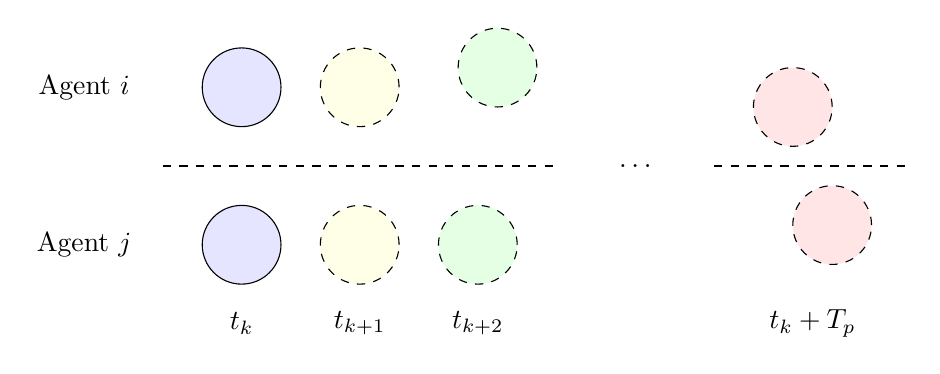
\begin{tikzpicture}[scale = 0.5]

  \draw[dashed] (0,0) -- (10,0);

  \node at (-2, 2) {Agent $i$};
  \node at (-2, -2) {Agent $j$};

  \filldraw[fill=blue!10!white, draw=black](2,2) circle (1cm);
  \filldraw[fill=blue!10!white, draw=black](2,-2) circle (1cm);
  \node at (2, -4) {$t_k$};


  \filldraw[fill=yellow!10!white, draw=black,dashed] (5,2) circle (1cm);
  \filldraw[fill=yellow!10!white, draw=black,dashed] (5,-2) circle (1cm);
  \node at (5, -4) {$t_{k+1}$};

  \filldraw[fill=green!10!white, draw=black,dashed] (8.5, 2.5) circle (1cm);
  \filldraw[fill=green!10!white, draw=black,dashed] (8,-2) circle (1cm);
  \node at (8, -4) {$t_{k+2}$};

  \node at (12, 0) {$\dots$};

  \draw[dashed] (14,0) -- (19,0);

  \filldraw[fill=red!10!white, draw=black,dashed] (16, 1.5) circle (1cm);
  \filldraw[fill=red!10!white, draw=black,dashed] (17,-1.5) circle (1cm);
  \node at (16.5, -4) {$t_k + T_p$};

\end{tikzpicture}

  \caption{The inter-agent constraint regime for two agents, $i,j$. Fully
    outlined circles denote measured configurations, while partly outlined
    circles denote predicted configurations. During the solution to the
    individual optimization problems, the predicted configuration of each agent
    at each timestep is constrained by the predicted configuration of the other
    agent at the same timestep (hence the homologously identical colours at
    each discrete timestep).}
  \label{fig:constraint_regime_horizon}
\end{figure}


The functions
$F_i : \mathcal{E}_{i,s} \times \mathcal{U}_i \to \mathbb{R}_{\geq 0}$ and
$V_i: \Omega_i \to \mathbb{R}_{\geq 0}$ are defined as
\begin{align}
  F_i \big(\overline{\vect{e}}_i(t), \overline{\vect{u}}_i(t)\big)
    &\triangleq \overline{\vect{e}}_i(t)^{\top} \mat{Q}_i \overline{\vect{e}}_i(t)
  + \overline{\vect{u}}_i(t)^{\top} \mat{R}_i \overline{\vect{u}}_i(t) \label{eq:F_i_def} \\[2.5ex]
  V_i \big(\overline{\vect{e}}_i(t)\big) & \triangleq \overline{\vect{e}}_i(t)^{\top} \mat{P}_i \overline{\vect{e}}_i(t) \label{eq:V_i_def}
\end{align}
Matrices $\mat{R}_i \in \mathbb{R}^{6 \times 6}$ and
$\mat{Q}_i, \mat{P}_i \in \mathbb{R}^{12 \times 12}$ are symmetric and positive
definite.  The running costs $F_i$ are upper- and lower-bounded by class
$\mathcal{K}_{\infty}$ functions:

\begin{bw_box}
  \begin{lemma} (\textit{$F_i$ is lower- and upper-bounded by class $\mathcal{K}_{\infty}$ functions})
    \label{lemma:F_i_bounded_K_class}

    Let functions $\alpha_1, \alpha_2 \in \mathcal{K}_{\infty}$ and $F_i$
    be defined by \eqref{eq:F_i_def}. Then, for all
    $\vect{e}_i \in \mathcal{E}_{i,s}$
    \begin{align}
      \alpha_1\big(\|\vect{e}_i\|\big) \leq F_i\big(\vect{e}_i, \vect{u}_i\big) \leq \alpha_2\big(\| \vect{e}_i \|\big)
    \end{align}
  \end{lemma}
\end{bw_box}


\begin{bw_box}
  \begin{lemma} ($F_i$ is Lipschitz continuous in $\mathcal{E}_{i,s} \times \mathcal{U}_i$)
\label{lemma:F_Lipschitz}

  Suppose that $\vect{e}_1, \vect{e}_2 \in \mathcal{E}_{i,s}$,
  $\vect{u}_i \in \mathcal{U}_i$ and that $F_i$ is defined by \eqref{eq:F_i_def}.
  The running costs $F_i$ are Lipschitz continuous in
  $\mathcal{E}_{i,s} \times \mathcal{U}_i$:
  $$\big|F_i(\vect{e}_1, \vect{u}_i) - F_i(\vect{e}_2, \vect{u}_i)\big| \leq L_{F_i} \|\vect{e}_1 - \vect{e}_2\|$$
  with Lipschitz constant $L_{F_i} = 2 \sigma_{max}(\mat{Q}_i) \overline{\varepsilon}_i $,
  where $\overline{\varepsilon}_i = \text{sup}\limits_{\vect{e}_i \in \mathcal{E}_{i,s}} \|\vect{e}_i\|$

\end{lemma}
\end{bw_box}


The terminal set $\Omega_i \subseteq \mathcal{E}_{i,t_k + T_p}$ is an admissible
positively invariant set according to definition
\eqref{def:positively_invariant} for system
\eqref{eq:position_based_error_model} such that
\begin{align}
  \Omega_i = \{\vect{e}_i \in \mathcal{E}_{i,t_k + T_p} : V_i(\vect{e}_i) \leq \varepsilon_{\Omega_i} \}
\end{align}
where $\varepsilon_{\Omega_i}$ is an arbitrarily small but fixed positive real scalar.

With regard to the terminal penalty function $V_i$, the following lemma will
prove to be useful in guaranteeing the convergence of the solution to the
optimal control problem to the terminal region $\Omega_i$:

\begin{bw_box}
\begin{lemma} ($V_i$ is Lipschitz continuous in $\Omega_i$)
\label{lemma:V_Lipschitz_e_0}

  Suppose that $\vect{e}_1, \vect{e}_2 \in \Omega_i$, and that
  $V_i$ is defined by \eqref{eq:V_i_def}. The terminal penalty function
  $V_i$ is Lipschitz continuous in $\Omega_i$
  $$\big|V_i(\vect{e}_1) - V_i(\vect{e}_2)\big| \leq L_{V_i} \|\vect{e}_1 - \vect{e}_2\|$$
  with Lipschitz constant $L_{V_i} = 2 \sigma_{max}(\mat{P}_i) \overline{\varepsilon}_{i,\Omega_i} $\\

  where $\overline{\varepsilon}_{i,\Omega_i} = \text{sup}\limits_{\vect{e}_i \in \Omega_i} \|\vect{e}_i\|$


\end{lemma}
\end{bw_box}


Furthermore, $V_i$ is lower- and upper-bounded by class $\mathcal{K}_{\infty}$ functions.

\begin{bw_box}
  \begin{lemma} (\textit{$V_i$ is lower- and upper-bounded by class
      \label{lemma:V_i_lower_upper_bounded}
    $\mathcal{K}_{\infty}$ functions in $\Omega_i$})
  \end{lemma}

  Let $\alpha_1, \alpha_2 \in \mathcal{K}_{\infty}$, $\vect{e}_i \in \Omega_i$
  and let $V_i$ be defined by \eqref{eq:V_i_def}. Then
  \begin{align}
    \alpha_1\big(\|\vect{e}_i\|\big) \leq V_i(\vect{e}_i) \leq \alpha_2\big(\| \vect{e}_i \|\big)
  \end{align}

\end{bw_box}


The solution to the optimal control problem \eqref{position_based_cost}
at time $t_k$ is an optimal control input, denoted by
$\overline{\vect{u}}_i^{\star}(\cdot;\ \vect{e}_i(t_k))$, which
is applied to the open-loop system until the next sampling instant $t_k + h$,
with $h \in (0,T_p)$:
\begin{align}
  %\vect{u}_i\big(t;\ \vect{e}_i(t_k)\big) = \overline{\vect{u}}_i^{\star}\big(t;\ \vect{e}_i(t_k)\big),\  t \in [t_k, t_k + h) \nonumber \\[2.5ex]
  \vect{u}_i(t) = \overline{\vect{u}}_i^{\star}\big(t;\ \vect{e}_i(t_k)\big),\  t \in [t_k, t_k + h]
 \label{eq:position_based_optimal_u}
\end{align}
At time $t_{k+1}$ a new finite horizon optimal control problem is solved in the
same manner, leading to a receding horizon approach.

The control input $\vect{u}_i(\cdot)$ is of feedback form,
since it is recalculated at each sampling instant based on the then-current
state. The solution to equation \eqref{eq:position_based_error_model} $-$ the
model of the real system, starting at time $t_1$, from an initial condition
$\vect{e}_i(t_1) = \overline{\vect{e}}_i(t_1)$,
by application of the control input $\vect{u}_i : [t_1, t_2] \to \mathcal{U}_i$
is denoted by
\begin{align}
  \vect{e}_i\big(t;\ \vect{u}_i(\cdot), \vect{e}_i(t_1)\big),\ t \in [t_1, t_2]
\end{align}


On the existence of solutions to \eqref{eq:position_based_error_model} we
assume the following:
\begin{bw_box}
\begin{assumption}
  \label{ass:existence_of_solutions_without_disturbance}

  The system \eqref{eq:position_based_error_model} has a
  \textit{continuous solution} for any $\vect{e}_i(0) \in \mathcal{E}_{i,0}$ and
  any \textit{piecewise continuous} input
  $\vect{u}_i(\cdot) :[0,T_p] \to \mathcal{U}_i$.
\end{assumption}
\end{bw_box}

The states of the open-loop system \eqref{eq:internal_error_model} $-$ the
predicted states obey the following notation:
\begin{bw_box}
\begin{remark}
The \textit{predicted} state of the system \eqref{eq:position_based_error_model}
at time $\tau \geq t_k$ , based on the measurement of the state at time
$t_k$, $\vect{e}_i(t_k)$, by application of the control input
\eqref{eq:position_based_optimal_u}, is denoted by
\begin{align}
  \overline{\vect{e}}_i\big(\tau;\ \vect{u}_i(\tau), \vect{e}_i(t_k)\big) \label{eq:position_based_predicted_error_0}
\end{align}
\end{remark}
\end{bw_box}

The closed-loop system for which stability is to be guaranteed is
\begin{align}
  \vect{e}_i(\tau) = g_i\big(\vect{e}_i(\tau), \overline{\vect{u}}_i^{\star}(\tau)\big),\ \tau \geq t_0 = 0
  \label{eq:without_disturbances_closed_loop}
\end{align}
where $\overline{\vect{u}}_i^{\star}(\tau) = \overline{\vect{u}}_i^{\star}(\tau;\ \vect{e}_i(t_k))$,
$\tau \in [t_k, t_k + h)$ and $t_0 = 0$.


We can now give the definition of an \textit{admissible input} for the FHOCP
\eqref{problem:opt_without_disturbances}:

\begin{bw_box}
  \begin{definition} (\textit{Admissible input for the FHOCP
\eqref{problem:opt_without_disturbances}})
  \label{definition:admissible_input}

  A control input $\vect{u}_i : [t_k, t_k + T_p] \to \mathbb{R}^6$ for a state
  $\vect{e}_i(t_k)$ is called \textit{admissible} for the problem
  \eqref{problem:opt_without_disturbances} if all the following hold:

  \begin{enumerate}
    \item $\vect{u}_i(\cdot)$ is piecewise continuous
    \item $\vect{u}_i(\tau) \in \mathcal{U}_i,\ \forall \tau \in [t_k, t_k + T_p]$
    \item $\overline{\vect{e}}_i\big(\tau;\ \vect{u}_i(\cdot), \vect{e}_i(t_k)\big) \in \mathcal{E}_{i,\tau},\ \forall \tau \in [t_k, t_k + T_p]$
    \item $\overline{\vect{e}}_i\big(t_k + T_p;\ \vect{u}_i(\cdot), \vect{e}_i(t_k)\big) \in \Omega_i$
  \end{enumerate}

  In other words, $\vect{u}_i$ is admissible if it conforms to the constraints
  on the input and its application yields states that conform to the
  prescribed state constraints of problem
  \eqref{problem:opt_without_disturbances} along the entire horizon
  $[t_k, t_k + T_p]$, and the terminal predicted state conforms to the
  terminal constraint.

\end{definition}
\end{bw_box}
